\clearpage

\section{Master conclusions}

This section is designed to draw general conclusions taking into account all modes of transport and their mode of survival. As the main factor is the CAPEX and knowing that this increases with the amount of traffic is taken into account the cost per Gbit/s calculated throughout this chapter. Through this we have a better idea of the cost of the network and it is possible to collect the best conclusions.

\begin{figure}[h!]
\centering
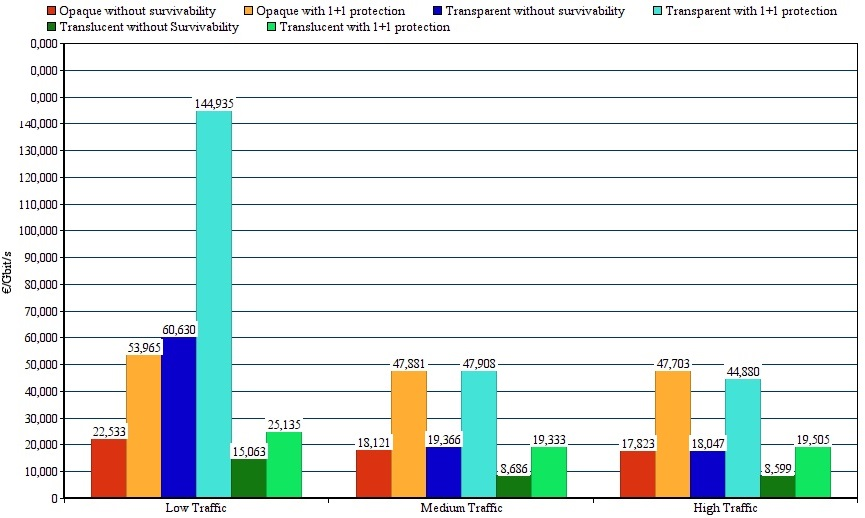
\includegraphics[width=\textwidth]{sdf/ilp/figures/comparative_image}
\caption{Graphic with the cost in Euros per Gbit/s of the three modes of transport without survivability and with 1+1 protection for all scenarios referred initially.}
\label{graphic_comparative}
\end{figure}

The first conclusion to draw from the previous chart is that regardless of the survival mode used and the amount of traffic the translucent transport mode is always better, ie it is always the lower cost.
Another important conclusion is that for all modes of transport without survivability and with 1+1 protection when the higher the network traffic the lower the cost per Gbit/s.
It should be noted that for survival mode with 1+1 protection for almost all the cases studied its cost is more than double the cost without survivability, only with the exemption of translucent mode for low traffic.
Looking only at the individual scenarios we can conclude that in the low scenario the transparent mode has a much higher cost compared to the other two transport modes for both modes of survival.
In relation to the other two scenarios it is possible to state that the opaque and transparent mode have a similar cost regardless of the mode of survivability.\\

The translucent mode has a much lower cost per Gbit/s than the other modes because this mode allows different pair $(o,d)$ to use the same optical channel thus decreasing the value of optical channels used and consequently decreases the CAPEX of the network.
The transparent mode has a very high cost per Gbit/s in the low scenario because this model, despite having little traffic, always defines at least one optical channel for each pair $(o,d)$ thus making the CAPEX of this network become very expensive.

